%%%%%%%%%%%%%%%%%%%%%%%%%%%%%%%%%%%%%%%%%%%%%%%%
% MAE 263F - Fall 2026 - SAMPLE Midterm 2: SOLUTIONS
% 31 multiple-choice questions (the actual midterm has 20 x 0.5 pts = 10 pts), 100 minutes
% Covers the whole course except Chapter 12 (Neural ODE), emphasizing topics not on Midterm 1:
% plates and shells (Ch. 9, HW4), hydrodynamics (Ch. 10), contact (Ch. 11), time integration (Ch. 2, 3, 6), HW1-HW3.
% Companion to SampleMidterm2_2026.tex (same questions and options).
%
% HOW TO EDIT:
%   Each question is one \sol{...} call:
%     \sol{<stem>}{<a>}{<b>}{<c>}{<d>}{<correct letter>}{<worked solution>}
%   The correct option is printed in bold with a check mark.
%   If you change a question in SampleMidterm2_2026.tex, update it here too.
%%%%%%%%%%%%%%%%%%%%%%%%%%%%%%%%%%%%%%%%%%%%%%%%

\documentclass[letterpaper,11pt]{article}

%%%%%%%%%%%%%%%%%%%%%%%%%%%%%%%%%%%%%%%%%%%%%%%%
% Packages
%%%%%%%%%%%%%%%%%%%%%%%%%%%%%%%%%%%%%%%%%%%%%%%%
\usepackage[top = 2.5cm, bottom = 2.5cm, left = 2.5cm, right = 2.5cm]{geometry}
\usepackage[T1]{fontenc}
\usepackage[utf8]{inputenc}
\usepackage{graphicx}
\usepackage{setspace}
\setlength{\parindent}{0in}
\usepackage{float}
\usepackage{fancyhdr}
\usepackage{lastpage}
\usepackage{physics}
\usepackage{gensymb}
\usepackage{comment}
\usepackage{enumitem}
\usepackage{amsmath,amssymb,amsfonts}
\usepackage[dvipsnames]{xcolor}
\usepackage{tikz}
\input{glyphtounicode}
\pdfgentounicode=1
\usepackage{url}
\usepackage[hidelinks]{hyperref}

\graphicspath{{figs/}}

%%%%%%%%%%%%%%%%%%%%%%%%%%%%%%%%%%%%%%%%%%%%%%%%
% Header and footer
%%%%%%%%%%%%%%%%%%%%%%%%%%%%%%%%%%%%%%%%%%%%%%%%
\pagestyle{fancy}
\fancyhf{}
\lhead{\footnotesize MAE-263F Sample Midterm 2: Solutions}
\rhead{\footnotesize \thepage \ of \pageref{LastPage}}
\lfoot{\footnotesize Copyright notice: Do not copy, distribute, republish, upload, post or transmit anything from the files hosted on the class website without written permission of the instructor}

%%%%%%%%%%%%%%%%%%%%%%%%%%%%%%%%%%%%%%%%%%%%%%%%
% Solution macro
%   \sol{stem}{a}{b}{c}{d}{correct letter}{worked solution}
%%%%%%%%%%%%%%%%%%%%%%%%%%%%%%%%%%%%%%%%%%%%%%%%
\newcounter{qnum}
\newcommand{\opt}[3]{\item \if#1#2{\boldmath\textbf{#3}} \quad \textcolor{OliveGreen}{\checkmark}\else #3\fi}
\newcommand{\sol}[7]{%
  \stepcounter{qnum}%
  \section*{Question \theqnum}
  #1
  \begin{enumerate}[label=(\alph*)]
    \opt{a}{#6}{#2}
    \opt{b}{#6}{#3}
    \opt{c}{#6}{#4}
    \opt{d}{#6}{#5}
  \end{enumerate}
  \vspace{1mm}
  \textbf{Answer: (#6)}

  \textbf{Solution.} #7

  \vspace{2mm}\hrule
}

%%%%%%%%%%%%%%%%%%%%%%%%%%%%%%%%%%%%%%%%%%%%%%%%
% Shared problem setups (repeated on each page of a question set)
%%%%%%%%%%%%%%%%%%%%%%%%%%%%%%%%%%%%%%%%%%%%%%%%
\newcommand{\hingesetup}{The hinge has four nodes (in meters): $\mathbf{x}_0 = [0, 0, 0]$, $\mathbf{x}_1 = [2, 0, 0]$, $\mathbf{x}_2 = [1, 1, 0]$, and $\mathbf{x}_3 = [1, -1, -1]$, shown below. Write each node as $\mathbf{x}_k = [x_k, y_k, z_k]$. The hinge edge is $\mathbf{x}_0$--$\mathbf{x}_1$; triangle~1 is $(\mathbf{x}_0, \mathbf{x}_1, \mathbf{x}_2)$ and triangle~2 is $(\mathbf{x}_0, \mathbf{x}_1, \mathbf{x}_3)$. The triangle normals are $\mathbf{n}_0 = (\mathbf{x}_1 - \mathbf{x}_0) \times (\mathbf{x}_2 - \mathbf{x}_0)$ and $\mathbf{n}_1 = (\mathbf{x}_3 - \mathbf{x}_0) \times (\mathbf{x}_1 - \mathbf{x}_0)$.
\begin{center}
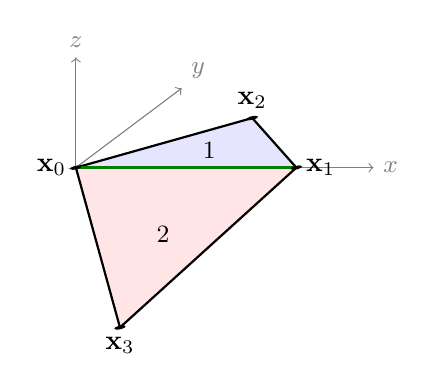
\begin{tikzpicture}[scale=1.4, x={(1cm,0cm)}, y={(0.6cm,0.45cm)}, z={(0cm,1cm)}]
  \draw[->, gray] (0,0,0) -- (2.7,0,0) node[right] {\small $x$};
  \draw[->, gray] (0,0,0) -- (0,1.6,0) node[above right] {\small $y$};
  \draw[->, gray] (0,0,0) -- (0,0,1.0) node[above] {\small $z$};
  \draw[thick, fill=blue!10] (0,0,0) -- (2,0,0) -- (1,1,0) -- cycle;
  \draw[thick, fill=red!10] (0,0,0) -- (2,0,0) -- (1,-1,-1) -- cycle;
  \draw[very thick, green!50!black] (0,0,0) -- (2,0,0);
  \foreach \p/\l/\a in {{(0,0,0)}/{\mathbf{x}_0}/left, {(2,0,0)}/{\mathbf{x}_1}/right, {(1,1,0)}/{\mathbf{x}_2}/above, {(1,-1,-1)}/{\mathbf{x}_3}/below} {
    \fill \p circle (0.045); \node[\a] at \p {$\l$};
  }
  \node at (1,0.35,0) {\small 1};
  \node at (1,-0.35,-0.45) {\small 2};
\end{tikzpicture}
\end{center}
}

\begin{document}

\thispagestyle{empty}

\noindent\begin{tabular}{@{}p{\linewidth}@{}}
{\large \bf Mechanics of Flexible Structures \& Soft Robots} \\
MAE-263F \\ Fall 2026 \\
\hline
\end{tabular}

\begin{center}
    {\LARGE \bf MAE-263F Sample Midterm 2: Solutions}
\end{center}

\textit{This sample midterm has 31 problems. The actual midterm will have 20 problems, each worth 0.5 pts.}

%
% Question 1
%
\sol{A rectangular plate with $4 \times 3$ nodes is meshed with 12 triangles as shown below (each square is cut by the diagonal from its lower-left to its upper-right corner).
\begin{center}
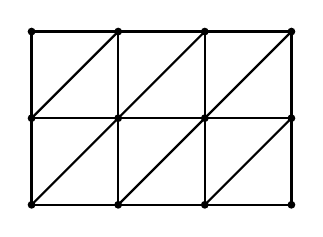
\begin{tikzpicture}[scale=1.1]
  \foreach \j in {0,1,2} { \draw[thick] (0,\j) -- (3,\j); }
  \foreach \i in {0,1,2,3} { \draw[thick] (\i,0) -- (\i,2); }
  \foreach \i in {0,1,2} { \foreach \j in {0,1} { \draw[thick] (\i,\j) -- (\i+1,\j+1); } }
  \foreach \i in {0,1,2,3} { \foreach \j in {0,1,2} { \fill (\i,\j) circle (0.045); } }
\end{tikzpicture}
\end{center}
How many edges and how many hinges does the mesh have?}
  {23 edges and 23 hinges}
  {17 edges and 7 hinges}
  {23 edges and 13 hinges}
  {26 edges and 13 hinges}
  {c}
  {Edges: $3 \times 3 = 9$ horizontal, $4 \times 2 = 8$ vertical, and $6$ diagonal, so $23$ edges. A hinge is an edge shared by two triangles; only the $2(3 + 2) = 10$ boundary edges are not. Hinges: $23 - 10 = 13$.}

%
% Question 2
%
\sol{Consider the following hinge. \hingesetup{}Compute the triangle normals $\mathbf{n}_0$ and $\mathbf{n}_1$.}
  {$\mathbf{n}_0 = [0, 0, 2]$, \ $\mathbf{n}_1 = [0, 2, -2]$}
  {$\mathbf{n}_0 = [0, 0, 2]$, \ $\mathbf{n}_1 = [0, -2, 2]$}
  {$\mathbf{n}_0 = [0, 0, 1]$, \ $\mathbf{n}_1 = [0, -1, -1]$}
  {$\mathbf{n}_0 = [2, 0, 0]$, \ $\mathbf{n}_1 = [0, -2, 2]$}
  {b}
  {$\mathbf{n}_0 = [2, 0, 0] \times [1, 1, 0] = [0 \cdot 0 - 0 \cdot 1, \; 0 \cdot 1 - 2 \cdot 0, \; 2 \cdot 1 - 0 \cdot 1] = [0, 0, 2]$. \\ $\mathbf{n}_1 = [1, -1, -1] \times [2, 0, 0] = [(-1)(0) - (-1)(0), \; (-1)(2) - (1)(0), \; (1)(0) - (-1)(2)] = [0, -2, 2]$. (Option (a) computes $\mathbf{e}^0 \times (\mathbf{x}_3 - \mathbf{x}_0)$ instead.)}

%
% Question 3
%
\sol{Consider the same hinge as in Question~2 (repeated here). \hingesetup{}The hinge angle $\theta$ is the signed angle from $\mathbf{n}_0$ to $\mathbf{n}_1$ about the hinge vector $\mathbf{e}^0 = \mathbf{x}_1 - \mathbf{x}_0$: it is positive if $\mathbf{n}_0 \times \mathbf{n}_1$ points along $\mathbf{e}^0$ and negative otherwise. What is $\theta$?}
  {$-\pi/4$}
  {$\pi/2$}
  {$3\pi/4$}
  {$\pi/4$}
  {d}
  {From Question~2, $\mathbf{n}_0 = [0, 0, 2]$ and $\mathbf{n}_1 = [0, -2, 2]$. $\cos\theta = \frac{\mathbf{n}_0 \cdot \mathbf{n}_1}{|\mathbf{n}_0| |\mathbf{n}_1|} = \frac{4}{2 \cdot 2\sqrt{2}} = \frac{1}{\sqrt{2}}$, so $|\theta| = \pi/4$. Sign: $\mathbf{n}_0 \times \mathbf{n}_1 = [4, 0, 0]$, which points along $\mathbf{e}^0 = [2, 0, 0]$. So $\theta = +\pi/4$.}

%
% Question 4
%
\sol{Consider the same hinge as in Questions~2--3 (repeated here), whose hinge angle is $\theta = \pi/4$. \hingesetup{}The bending stiffness is $k_b = 2\,\mathrm{N\,m}$ and the bending energy is $E_b = \frac{1}{2} k_b (\theta - \bar{\theta})^2$. What is $E_b$ if the hinge is a \emph{plate} ($\bar{\theta} = 0$), and if it is a \emph{shell} with $\bar{\theta} = \pi/6$?}
  {Plate: $\pi^2/8\,\mathrm{J}$; shell: $\pi^2/72\,\mathrm{J}$}
  {Plate: $\pi^2/16\,\mathrm{J}$; shell: $25\pi^2/144\,\mathrm{J}$}
  {Plate: $\pi^2/16\,\mathrm{J}$; shell: $\pi^2/144\,\mathrm{J}$}
  {Plate: $\pi/4\,\mathrm{J}$; shell: $\pi/12\,\mathrm{J}$}
  {c}
  {Plate: $E_b = \frac{1}{2} \cdot 2 \cdot (\pi/4)^2 = \pi^2/16\,\mathrm{J}$. Shell: $E_b = \frac{1}{2} \cdot 2 \cdot (\pi/4 - \pi/6)^2 = (\pi/12)^2 = \pi^2/144\,\mathrm{J}$. (Option (b) uses $\theta + \bar{\theta} = 5\pi/12$.)}

%
% Question 5
%
\sol{Consider a setup similar to Question~4 (repeated here): a \emph{plate} ($\bar{\theta} = 0$) with $k_b = 2\,\mathrm{N\,m}$ and $E_b = \frac{1}{2} k_b \theta^2$. \hingesetup{}Node $\mathbf{x}_3$ is now moved from $[1, -1, -1]$ to $[1, 0, -1]$, and all other nodes stay where they are. What is the new bending energy $E_b$?}
  {$\pi^2/4\,\mathrm{J}$}
  {$0$}
  {$\pi^2/16\,\mathrm{J}$}
  {$\pi^2/2\,\mathrm{J}$}
  {a}
  {$\mathbf{n}_1 = [1, 0, -1] \times [2, 0, 0] = [0, -2, 0]$, which is perpendicular to $\mathbf{n}_0 = [0, 0, 2]$; $\mathbf{n}_0 \times \mathbf{n}_1 = [4, 0, 0]$ points along $\mathbf{e}^0$, so $\theta = \pi/2$. $E_b = \frac{1}{2} \cdot 2 \cdot (\pi/2)^2 = \pi^2/4\,\mathrm{J}$.}

%
% Question 6
%
\sol{Consider the same hinge as in Questions~2--4 (repeated here), as a plate with $E_b = \frac{1}{2} k_b \theta^2$. \hingesetup{}Which component of the gradient of the bending energy is \textbf{zero}?}
  {$\partial E_b / \partial y_3$}
  {$\partial E_b / \partial z_0$}
  {$\partial E_b / \partial z_2$}
  {$\partial E_b / \partial y_2$}
  {d}
  {Triangle~1 lies in the plane $z = 0$. Moving $\mathbf{x}_2$ in $y$ keeps it in that plane, so $\mathbf{n}_0$ keeps its direction; $\mathbf{n}_1$ does not depend on $\mathbf{x}_2$. Thus $\theta$, and therefore $E_b$, do not change: $\partial E_b / \partial y_2 = 0$. Moving $\mathbf{x}_3$ in $y$, $\mathbf{x}_0$ in $z$, or $\mathbf{x}_2$ in $z$ tilts a triangle and changes $\theta$, so those components are nonzero. (From \texttt{gradEb\_hessEb\_Shell}: $\partial E_b/\partial y_3 = \pi/4$, $\partial E_b/\partial z_0 = 3\pi/8$, $\partial E_b/\partial z_2 = -\pi/2$.)}

%
% Question 7
%
\sol{Let $\mathbf{f}(x, y) = \begin{bmatrix} f_1 \\ f_2 \end{bmatrix} = \begin{bmatrix} x^2 + 3y \\ x y^2 \end{bmatrix}$. At $(x, y) = (1, 1)$, estimate the Jacobian $J_{ij} = \partial f_i / \partial q_j$ (with $q_1 = x$, $q_2 = y$) using the forward finite difference \[ \frac{\partial f_i}{\partial q_j} \approx \frac{f_i(\mathbf{q} + \Delta q\, \mathbf{e}_j) - f_i(\mathbf{q})}{\Delta q}, \] where $\mathbf{e}_j$ perturbs only $q_j$, with $\Delta q = 0.1$. That is, perturb $x$ to $1.1$ (keeping $y = 1$) for the first column, and perturb $y$ to $1.1$ (keeping $x = 1$) for the second column. What is the finite-difference estimate of $\mathbf{J}$?}
  {$\begin{bmatrix} 2 & 3 \\ 1 & 2 \end{bmatrix}$}
  {$\begin{bmatrix} 2.1 & 1 \\ 3 & 2.1 \end{bmatrix}$}
  {$\begin{bmatrix} 0.21 & 0.3 \\ 0.1 & 0.21 \end{bmatrix}$}
  {$\begin{bmatrix} 2.1 & 3 \\ 1 & 2.1 \end{bmatrix}$}
  {d}
  {$\mathbf{f}(1, 1) = [4, 1]^T$. Perturbing $x$: $\mathbf{f}(1.1, 1) = [1.21 + 3, \; 1.1]^T = [4.21, 1.1]^T$, so the first column is $([4.21, 1.1]^T - [4, 1]^T)/0.1 = [2.1, 1]^T$. Perturbing $y$: $\mathbf{f}(1, 1.1) = [1 + 3.3, \; 1.21]^T = [4.3, 1.21]^T$, so the second column is $[3, 2.1]^T$. The exact Jacobian is $\begin{bmatrix} 2x & 3 \\ y^2 & 2xy \end{bmatrix} = \begin{bmatrix} 2 & 3 \\ 1 & 2 \end{bmatrix}$ (option (a)); the finite difference is off by $0.1$ in the entries that depend on the perturbed variable.}

%
% Question 8
%
\sol{An edge of a plate has undeformed length $l = 0.1\,\mathrm{m}$. The plate has Young's modulus $Y = 1\,\mathrm{MPa}$ and thickness $h = 1\,\mathrm{mm}$, so $k_s = \frac{\sqrt{3}}{2} Y h l^2 = 5\sqrt{3}\,\mathrm{N\,m}$. The edge is stretched to a length of $0.11\,\mathrm{m}$. What is its stretching energy $E_s = \frac{1}{2} k_s \left( \frac{\|\mathbf{e}\|}{l} - 1 \right)^2$?}
  {$\sqrt{3}/20\,\mathrm{J}$}
  {$\sqrt{3}/40\,\mathrm{J}$}
  {$\sqrt{3}/4\,\mathrm{J}$}
  {$\sqrt{3}/4000\,\mathrm{J}$}
  {b}
  {Strain: $0.11/0.1 - 1 = 0.1$. $E_s = \frac{1}{2} \cdot 5\sqrt{3} \cdot 0.1^2 = \frac{5\sqrt{3}}{200} = \frac{\sqrt{3}}{40}\,\mathrm{J}$. (Option (d) uses the change in length, $0.01\,\mathrm{m}$, as if it were the strain.)}

%
% Question 9
%
\sol{The thickness $h$ of a plate is doubled. By what factors do the bending stiffness $k_b = \frac{2}{\sqrt{3}} \frac{Y h^3}{12}$ and the stretching stiffness $k_s = \frac{\sqrt{3}}{2} Y h l^2$ change?}
  {Both double.}
  {Both increase by a factor of 8.}
  {$k_b$ doubles; $k_s$ increases by a factor of 8.}
  {$k_b$ increases by a factor of 8; $k_s$ doubles.}
  {d}
  {$k_b \propto h^3$, so it increases by $2^3 = 8$; $k_s \propto h$, so it doubles. This is why thin plates and shells bend easily but resist stretching.}

%
% Question 10
%
\sol{A discrete plate has $N$ nodes. How many DOFs does it have, and what are the sizes of the gradient vector of one hinge's bending energy and of one edge's stretching energy?}
  {$3N$ DOFs; hinge gradient: 12; edge gradient: 6}
  {$4N - 1$ DOFs; hinge gradient: 12; edge gradient: 6}
  {$3N$ DOFs; hinge gradient: 9; edge gradient: 6}
  {$3N$ DOFs; hinge gradient: 12; edge gradient: 3}
  {a}
  {Each node has three coordinates and there are no twist angles, so the DOF vector has $3N$ entries ($4N - 1$ is the DER rod). The bending energy of a hinge depends on four nodes ($12$ DOFs), and the stretching energy of an edge on two nodes ($6$ DOFs); \texttt{gradEb\_hessEb\_Shell} returns a 12-vector and a $12 \times 12$ Hessian.}

%
% Question 11
%
\sol{In a discrete shell simulation, how is the natural hinge angle $\bar{\theta}$ of each hinge obtained?}
  {It is recomputed at every time step from the current shape.}
  {It is computed once, from the initial (undeformed) shape, before time stepping starts; for a plate, it is zero.}
  {It is zero for every hinge of a shell.}
  {It is a degree of freedom solved for by Newton's method.}
  {b}
  {The natural hinge angles $\bar{\theta}_k$ (and the undeformed edge lengths) are computed once from the undeformed configuration, usually $\mathbf{q}(0)$, and stored before time stepping. For a plate, the undeformed shape is flat, so $\bar{\theta}_k = 0$; for a shell, $\bar{\theta}_k \neq 0$ in general.}

%
% Question 12
%
\sol{A discrete shell has four nodes, $\mathbf{x}_0$, $\mathbf{x}_1$, $\mathbf{x}_2$, $\mathbf{x}_3$, each with three coordinates. Its DOF vector is $\mathbf{q} = [\mathbf{x}_0, \mathbf{x}_1, \mathbf{x}_2, \mathbf{x}_3]$ (size 12, Python indices 0--11), so node $\mathbf{x}_k$ occupies \texttt{q[3*k : 3*k+3]}. Nodes $\mathbf{x}_0$, $\mathbf{x}_1$, $\mathbf{x}_2$ are clamped (fixed) and $\mathbf{x}_3$ is free. Which Python indices of $\mathbf{q}$ are the free DOFs?}
  {\texttt{0, 1, 2}}
  {\texttt{0} through \texttt{8}}
  {\texttt{9, 10, 11}}
  {All 12 indices}
  {c}
  {Node $\mathbf{x}_3$ occupies \texttt{q[9:12]}, so \texttt{freeIndex = np.arange(9, 12)}, i.e., indices 9, 10, 11. Only these rows and columns of $\mathbf{f}$ and $\mathbf{J}$ are solved.}

%
% Question 13
%
\sol{In resistive force theory, the drag on a rod depends on the direction of motion: moving along the rod is resisted less than moving sideways. So the velocity $\mathbf{v}$ (a column vector) of a node is decomposed into a tangential velocity $\mathbf{v}_t$, along the unit tangent $\mathbf{t}$ (a column vector), and a normal velocity $\mathbf{v}_n$, perpendicular to $\mathbf{t}$, with $\mathbf{v} = \mathbf{v}_t + \mathbf{v}_n$. What is $\mathbf{v}_t$?}
  {$(\mathbf{t}^T \mathbf{t})\, \mathbf{v}$}
  {$(\mathbf{I} - \mathbf{t}\mathbf{t}^T)\, \mathbf{v}$}
  {$\mathbf{t} \times \mathbf{v}$}
  {$(\mathbf{t}\mathbf{t}^T)\, \mathbf{v}$}
  {d}
  {$(\mathbf{t}\mathbf{t}^T)\mathbf{v} = \mathbf{t}(\mathbf{t}^T\mathbf{v}) = (\mathbf{t} \cdot \mathbf{v})\,\mathbf{t}$, the projection of $\mathbf{v}$ onto $\mathbf{t}$ ($\mathbf{P}_t = \mathbf{t}\mathbf{t}^T$, Eq.~10.7). Option (b) is the normal component; option (a) is just $\mathbf{v}$ because $\mathbf{t}^T\mathbf{t} = 1$.}

%
% Question 14
%
\sol{As in Question~13, the velocity $\mathbf{v}$ of a node of a rod is decomposed into a tangential velocity $\mathbf{v}_t$ (along the unit tangent $\mathbf{t}$) and a normal velocity $\mathbf{v}_n$ (perpendicular to $\mathbf{t}$), with $\mathbf{v} = \mathbf{v}_t + \mathbf{v}_n$. For $\mathbf{t} = [0.6, 0.8, 0]^T$ and $\mathbf{v} = [1, 2, 0]^T\,\mathrm{m/s}$, what is the normal velocity $\mathbf{v}_n$?}
  {$[1.32, 1.76, 0]^T\,\mathrm{m/s}$}
  {$[-0.32, 0.24, 0]^T\,\mathrm{m/s}$}
  {$[0.32, -0.24, 0]^T\,\mathrm{m/s}$}
  {$[0.4, 1.2, 0]^T\,\mathrm{m/s}$}
  {b}
  {$\mathbf{v}_n = (\mathbf{I} - \mathbf{t}\mathbf{t}^T)\,\mathbf{v} = \mathbf{v} - (\mathbf{t} \cdot \mathbf{v})\,\mathbf{t}$. Here $\mathbf{t} \cdot \mathbf{v} = 0.6 + 1.6 = 2.2$, so $\mathbf{v}_t = 2.2\,\mathbf{t} = [1.32, 1.76, 0]^T$ and $\mathbf{v}_n = [1, 2, 0]^T - [1.32, 1.76, 0]^T = [-0.32, 0.24, 0]^T$. Check: it is perpendicular to $\mathbf{t}$ ($-0.192 + 0.192 = 0$).}

%
% Question 15
%
\sol{In resistive force theory, the drag on node $k$ is $\mathbf{f}_k = -l_k \left( C_t \mathbf{P}_t + C_p \mathbf{P}_n \right) \mathbf{u}_k$, with $\mathbf{P}_t = \mathbf{t}\mathbf{t}^T$ and $\mathbf{P}_n = \mathbf{I} - \mathbf{P}_t$. Let $l_k = 0.01\,\mathrm{m}$, $C_t = 1$, $C_p = 2$ (in $\mathrm{Pa \cdot s}$), $\mathbf{t} = [1, 0, 0]^T$, and $\mathbf{u}_k = [0.1, 0.1, 0]^T\,\mathrm{m/s}$ (no background flow). What is $\mathbf{f}_k$?}
  {$[-0.001, -0.002, 0]^T\,\mathrm{N}$}
  {$[-0.002, -0.001, 0]^T\,\mathrm{N}$}
  {$[0.001, 0.002, 0]^T\,\mathrm{N}$}
  {$[-0.1, -0.2, 0]^T\,\mathrm{N}$}
  {a}
  {Tangential part of $\mathbf{u}_k$: $[0.1, 0, 0]^T$; normal part: $[0, 0.1, 0]^T$. $\mathbf{f}_k = -0.01\,(1 \cdot [0.1, 0, 0]^T + 2 \cdot [0, 0.1, 0]^T) = [-0.001, -0.002, 0]^T\,\mathrm{N}$. Moving sideways costs twice as much drag as moving along the rod.}

%
% Question 16
%
\sol{At high Reynolds number, the drag on node $k$ of a rod is $\mathbf{f}_k = -k_k \|\mathbf{u}^{\text{rel}}_k\| \, \mathbf{u}^{\text{rel}}_k$. Here $\mathbf{u}^{\text{rel}}_k = \mathbf{u}_k - \mathbf{U}_\infty$ is the velocity of the node relative to the background flow, and $k_k = \frac{1}{2} \rho C_D A_k$ is a constant that depends on the fluid density $\rho$, the drag coefficient $C_D$, and the projected area $A_k$ of the rod segment around node $k$. If the relative velocity is tripled (same direction), by what factor does the magnitude of the drag force change?}
  {3}
  {6}
  {9}
  {27}
  {c}
  {$\|\mathbf{f}_k\| = k_k \|\mathbf{u}^{\text{rel}}_k\|^2$, so tripling the speed multiplies the drag by $3^2 = 9$. (In the low-Re model the drag is linear, so it would only triple.)}

%
% Question 17
%
\sol{A rod of diameter $L = 0.01\,\mathrm{m}$ moves at $v = 1\,\mathrm{m/s}$ in water ($\rho = 1000\,\mathrm{kg/m^3}$, $\mu = 10^{-3}\,\mathrm{Pa \cdot s}$). What is the Reynolds number $Re = \rho v L / \mu$, and which hydrodynamic model is appropriate?}
  {$Re = 10$; resistive force theory (low Re)}
  {$Re = 10^4$; resistive force theory (low Re)}
  {$Re = 10^{-4}$; quadratic drag (high Re)}
  {$Re = 10^4$; quadratic drag (high Re)}
  {d}
  {$Re = 1000 \cdot 1 \cdot 0.01 / 10^{-3} = 10^4 \gg 1$: inertial effects dominate, so the quadratic (high-Re) drag model is appropriate.}

%
% Question 18
%
\sol{A rod has nodes $\mathbf{x}_0, \mathbf{x}_1, \ldots, \mathbf{x}_{N-1}$. The two end nodes, $\mathbf{x}_0$ and $\mathbf{x}_{N-1}$, belong to only one edge each; all other nodes are \emph{interior} nodes and belong to two edges (the edge before and the edge after). The tangent at an interior node $\mathbf{x}_k$ is the normalized average of the unit tangents of these two edges. For an interior node with $\mathbf{x}_k - \mathbf{x}_{k-1} = [2, 0, 0]$ and $\mathbf{x}_{k+1} - \mathbf{x}_k = [0, 3, 0]$, what is the node tangent?}
  {$\frac{1}{\sqrt{2}}[1, 1, 0]$}
  {$\frac{1}{\sqrt{13}}[2, 3, 0]$}
  {$[1, 1, 0]$}
  {$[0, 1, 0]$}
  {a}
  {Unit edge tangents: $[1, 0, 0]$ and $[0, 1, 0]$. Their sum is $[1, 1, 0]$, and normalizing gives $\frac{1}{\sqrt{2}}[1, 1, 0]$. Option (b) adds the edges before normalizing them, which weights the longer edge more.}

%
% Question 19
%
\sol{In the predictor--corrector method, a node is held fixed on the ground. After the solve, its reaction force points \emph{toward} the ground, i.e., the ground would have to pull the node down to keep it there. What should the algorithm do?}
  {Keep the node fixed, because it is already on the ground.}
  {Release the node (make its vertical DOF free again), because the ground can only push, not pull, and then do a corrector solve.}
  {Move the node below the ground to balance the force.}
  {Nothing; reaction forces do not affect the contact constraints.}
  {b}
  {Ground contact can only push. A reaction that pulls the node toward the ground would be an adhesive force, so the constraint is released (Eq.~11.11). Because the set of constraints changed, a corrector solve is needed.}

%
% Question 20
%
\sol{Two masses hang in a chain: spring $k_1 = 30\,\mathrm{N/m}$ connects a fixed support to mass $m_1 = 1\,\mathrm{kg}$, and spring $k_2 = 30\,\mathrm{N/m}$ connects $m_1$ to mass $m_2 = 2\,\mathrm{kg}$. Gravity is $g = 10\,\mathrm{m/s^2}$. At static equilibrium, what is the displacement of $m_2$ from its position when both springs are unstretched?}
  {$1.00\,\mathrm{m}$}
  {$2.00\,\mathrm{m}$}
  {$1.67\,\mathrm{m}$}
  {$0.67\,\mathrm{m}$}
  {c}
  {Spring~1 carries the weight of both masses, $(1 + 2) \cdot 10 = 30\,\mathrm{N}$, so it stretches $1\,\mathrm{m}$. Spring~2 carries only $m_2$: $20\,\mathrm{N}$, so it stretches $2/3\,\mathrm{m}$. The displacement of $m_2$ is $1 + 2/3 = 1.67\,\mathrm{m}$.}

%
% Question 21
%
\sol{A mass $m$ is attached to a spring of stiffness $k$ (no damping, no gravity). Its position $x(t)$ obeys \[ m \ddot{x} + k x = 0. \] Writing the velocity as $u = \dot{x}$, this is the first-order system $\dot{x} = u$ and $\dot{u} = a$, where $a = -k x / m$ is the acceleration. The \emph{explicit} Euler method advances from time $t$ to $t + \Delta t$ using only the known (old) values at time $t$: \[ x^{\text{new}} = x^{\text{old}} + \Delta t\, u^{\text{old}}, \qquad u^{\text{new}} = u^{\text{old}} + \Delta t\, a^{\text{old}}, \qquad a^{\text{old}} = -k x^{\text{old}} / m. \] Let $m = 1\,\mathrm{kg}$, $k = 100\,\mathrm{N/m}$, and $\Delta t = 0.01\,\mathrm{s}$. The mass starts at $x^{\text{old}} = 0.1\,\mathrm{m}$ with $u^{\text{old}} = 0$. After one explicit Euler step, what are $x^{\text{new}}$ and $u^{\text{new}}$?}
  {$x = 0.099\,\mathrm{m}$, $u = -0.1\,\mathrm{m/s}$}
  {$x = 0.1\,\mathrm{m}$, $u = 0$}
  {$x = 0.09\,\mathrm{m}$, $u = -1\,\mathrm{m/s}$}
  {$x = 0.1\,\mathrm{m}$, $u = -0.1\,\mathrm{m/s}$}
  {d}
  {$x^{\text{new}} = 0.1 + 0.01 \cdot 0 = 0.1\,\mathrm{m}$. $a^{\text{old}} = -100 \cdot 0.1 / 1 = -10\,\mathrm{m/s^2}$, so $u^{\text{new}} = 0 + 0.01 \cdot (-10) = -0.1\,\mathrm{m/s}$. Both updates use only old values.}

%
% Question 22
%
\sol{An undamped mass--spring system is simulated with explicit Euler (as in Question~21) with any time step $\Delta t$. What happens to the oscillation over a long simulation?}
  {Its amplitude grows without bound.}
  {Its amplitude decays to zero.}
  {It matches the exact solution.}
  {The mass stays at its initial position.}
  {a}
  {Explicit Euler adds energy to an undamped oscillator at every step, so the amplitude grows without bound (HW1, Question~10). Implicit Euler does the opposite: it removes energy.}

%
% Question 23
%
\sol{An undamped mass--spring system is simulated with implicit Euler, and its oscillation slowly dies out. What happens if the time step $\Delta t$ is made smaller?}
  {The oscillation dies out faster.}
  {The oscillation dies out more slowly, because the artificial damping is weaker.}
  {Nothing changes; the artificial damping does not depend on $\Delta t$.}
  {The simulation becomes unstable.}
  {b}
  {Implicit Euler's artificial (numerical) damping decreases as $\Delta t$ decreases, so the oscillation persists longer and is closer to the exact (undamped) solution (HW1, Question~9).}

%
% Question 24
%
\sol{The Newmark--Beta method advances the position $x$, velocity $\dot{x}$, and acceleration $\ddot{x}$ from time step $n$ to $n+1$ (step size $\Delta t$) using \[ x_{n+1} = x_n + \Delta t\, \dot{x}_n + \Delta t^2 \left[ \left( \tfrac{1}{2} - \beta \right) \ddot{x}_n + \beta\, \ddot{x}_{n+1} \right], \qquad \dot{x}_{n+1} = \dot{x}_n + \Delta t \left[ (1 - \gamma)\, \ddot{x}_n + \gamma\, \ddot{x}_{n+1} \right], \] where $\beta$ and $\gamma$ are parameters that weight the old acceleration $\ddot{x}_n$ against the new one $\ddot{x}_{n+1}$. Which choice of $\beta$ and $\gamma$ is unconditionally stable but \emph{strongly dissipative} (the energy of an undamped oscillator decays, similar to implicit Euler)?}
  {$\beta = 0.25$, $\gamma = 0.5$}
  {$\beta = 0$, $\gamma = 0.5$}
  {$\beta = 0.5$, $\gamma = 1.0$}
  {All choices conserve energy.}
  {c}
  {$\beta = 0.5$, $\gamma = 1.0$ is the fully implicit Newmark method: unconditionally stable but strongly dissipative (Ch.~6.2). $\beta = 0.25$, $\gamma = 0.5$ (average acceleration) is time-symmetric and conserves energy for undamped linear systems.}

%
% Question 25
%
\sol{A metal sphere ($\rho_{\text{metal}} = 7000\,\mathrm{kg/m^3}$) is released from rest in a fluid ($\rho_{\text{fluid}} = 1000\,\mathrm{kg/m^3}$) with no viscosity. With $g = 9.8\,\mathrm{m/s^2}$, what is its speed after $2\,\mathrm{s}$?}
  {$19.6\,\mathrm{m/s}$}
  {$16.8\,\mathrm{m/s}$}
  {$2.8\,\mathrm{m/s}$}
  {$8.4\,\mathrm{m/s}$}
  {b}
  {Net downward force $= \frac{4}{3}\pi R^3 (\rho_{\text{metal}} - \rho_{\text{fluid}}) g$ and mass $= \frac{4}{3}\pi R^3 \rho_{\text{metal}}$, so $a = g\,(1 - 1000/7000) = 8.4\,\mathrm{m/s^2}$ and $v = 8.4 \cdot 2 = 16.8\,\mathrm{m/s}$.}

%
% Question 26
%
\sol{A metal sphere of radius $R = 0.01\,\mathrm{m}$ ($\rho_{\text{metal}} = 10000\,\mathrm{kg/m^3}$) falls in a viscous fluid ($\rho_{\text{fluid}} = 1000\,\mathrm{kg/m^3}$, $\mu = 1000\,\mathrm{Pa \cdot s}$) with $g = 10\,\mathrm{m/s^2}$. The drag is $6\pi\mu R v$. What is the terminal speed?}
  {$2 \times 10^{-3}\,\mathrm{m/s}$}
  {$2.2 \times 10^{-3}\,\mathrm{m/s}$}
  {$9 \times 10^{-3}\,\mathrm{m/s}$}
  {$2 \times 10^{-1}\,\mathrm{m/s}$}
  {a}
  {At terminal speed, $6\pi\mu R v = \frac{4}{3}\pi R^3 (\rho_{\text{metal}} - \rho_{\text{fluid}}) g$, so $v = \frac{2}{9}\frac{(\rho_{\text{metal}} - \rho_{\text{fluid}}) g R^2}{\mu} = \frac{2}{9} \cdot \frac{9000 \cdot 10 \cdot 10^{-4}}{1000} = \frac{2}{9} \cdot 9 \times 10^{-3} = 2 \times 10^{-3}\,\mathrm{m/s}$. (Option (b) ignores buoyancy, using $\rho_{\text{metal}}$ instead of $\rho_{\text{metal}} - \rho_{\text{fluid}}$; option (c) forgets the factor $\frac{2}{9}$; option (d) uses $R$ instead of $R^2$.)}

%
% Question 27
%
\sol{A cantilever of free length $L = 0.1\,\mathrm{m}$, circular cross-section of radius $r_0 = 1\,\mathrm{mm}$, Young's modulus $E = 1\,\mathrm{GPa}$, and density $\rho = 1000\,\mathrm{kg/m^3}$ sags under its own weight ($g = 10\,\mathrm{m/s^2}$). What is the Euler--Bernoulli tip deflection $\delta = q L^4 / (8EI)$, with $q = \rho A g$?}
  {$4.0\,\mathrm{mm}$}
  {$0.25\,\mathrm{mm}$}
  {$2.0\,\mathrm{mm}$}
  {$0.5\,\mathrm{mm}$}
  {d}
  {With $A = \pi r_0^2$ and $I = \pi r_0^4/4$: $\delta = \frac{\rho g L^4}{2 E r_0^2} = \frac{1000 \cdot 10 \cdot 10^{-4}}{2 \cdot 10^9 \cdot 10^{-6}} = 5 \times 10^{-4}\,\mathrm{m} = 0.5\,\mathrm{mm}$.}

%
% Question 28
%
\sol{In the small-deflection regime, the free length of the cantilever in Question~27 is doubled (all else unchanged). By what factor does the tip deflection change?}
  {2}
  {4}
  {16}
  {8}
  {c}
  {$\delta = q L^4/(8EI)$, and $q$ (weight per unit length) does not change, so $\delta \propto L^4$: doubling $L$ multiplies $\delta$ by $2^4 = 16$.}

%
% Question 29
%
\sol{A horizontal cantilever of length $L$ is clamped at one end and sags under its own weight (a uniform load $q$ per unit length). Euler--Bernoulli beam theory predicts the tip deflection $\delta_{\text{EB}} = qL^4/(8EI)$, which grows linearly with $q$ and can even exceed $L$ for a large enough load. A DER simulation with a large load gives a vertical tip deflection much smaller than $\delta_{\text{EB}}$ (and always less than $L$). What is the main reason for the difference?}
  {Euler--Bernoulli theory is linear: it assumes small slopes and a shape that stays close to the undeformed one. DER makes no such assumption.}
  {Implicit Euler adds artificial damping that reduces the DER deflection.}
  {The rod stretches a lot at large loads.}
  {DER includes inertia, while Euler--Bernoulli theory does not.}
  {a}
  {Euler--Bernoulli theory is geometrically linear (small slopes, fixed geometry), so its deflection is linear in the load and overpredicts large deflections (it can even predict a deflection larger than $L$). DER is geometrically nonlinear: as the rod rotates toward the vertical, the moment arm of the weight shrinks and the vertical deflection saturates below $L$. At steady state, damping and inertia do not affect the shape, and stretching is negligible.}

%
% Question 30
%
\sol{In DER, the bending energy at node $k$ is $\frac{1}{2} EI\, |\boldsymbol{\kappa}_k - \bar{\boldsymbol{\kappa}}_k|^2 / \bar{l}_k$, where $\boldsymbol{\kappa}_k$ is the curvature and $\bar{\boldsymbol{\kappa}}_k$ is the natural (stress-free) curvature, and $\bar{l}_k$ is the undeformed Voronoi length of node $k$. A rod clamped at one end is initialized in the shape of a circular arc, and there is no gravity or other load. Normally $\bar{\boldsymbol{\kappa}}$ is computed from this initial shape, which makes the rod naturally curved. Instead, a student sets $\bar{\boldsymbol{\kappa}}_k = \mathbf{0}$ at every node (a naturally straight rod) but still starts the simulation from the circular arc. What happens?}
  {It keeps its curved shape, because there is no load.}
  {It opens up into a nearly straight rod, because the bending energy is zero only when the rod is straight.}
  {It curls up more tightly.}
  {The simulation fails, because the natural curvature must not be zero.}
  {b}
  {The bending energy $\frac{1}{2}EI|\boldsymbol{\kappa}_k - \bar{\boldsymbol{\kappa}}_k|^2/\bar{l}_k$ is zero only when $\boldsymbol{\kappa}_k = \bar{\boldsymbol{\kappa}}_k$. With $\bar{\boldsymbol{\kappa}} = \mathbf{0}$, the stress-free shape is straight, so the rod, started from the arc, opens up into a nearly straight rod (HW3, Question~11).}

%
% Question 31
%
\sol{Use $x$, $y$, $z$ coordinates with gravity along $-z$. The two rods described below are both clamped at one end and simulated with DER. Rod A is naturally straight and initially lies along the $x$-axis. Rod B is naturally curved: its stress-free shape is a circular arc in the $x$--$y$ (horizontal) plane, and it starts in that shape. Both rods sag under gravity. Which statement about their twist angles is true?}
  {Both rods twist, because gravity always twists a rod.}
  {Neither rod twists, because the first twist angle is fixed.}
  {Rod A does not twist (it bends only in the $x$--$z$ plane that contains it); rod B twists (gravity bends it out of the $x$--$y$ plane in which it is curved).}
  {Rod A twists, but rod B does not.}
  {c}
  {Rod A bends within the vertical $x$--$z$ plane that contains it, so its twist angles stay zero. Rod B is curved in the horizontal $x$--$y$ plane and gravity pulls it out of that plane (along $-z$), which couples bending and twisting, so it develops nonzero twist (HW3, Question~10).}

\end{document}
